% \theoremstyle{definition}
\newtheorem{definition}{Definition}[section]
본 연구의 연구 흐름에 대해 기술하는 장이다. motivation부터 연구를 이해하는데 필요한 배경 지식, 본 연구의 필요성 등이 논리적으로 함유되었다.
\section{Motivation}
\subsection{NeRF and QRF}
\textit{설명(삭제예정) : 컴퓨터 비전(상당히 대중적인 주제)의 문제로부터 양자머신러닝 모델의 잠재력을 어필하는 장이다.}

% 컴퓨터 비전 분야에서, 특정 객체에 대한 여러 사진을 Input으로 하여, 입력되지 않은 새로운 view에서의 객체의 형상을 모델링하는 task는 굉장히 중요한 문제이다. view synthesis라고 불리는 이 작업은, 기존에는 해당 객체를 포함한 공간(보통은 3D)의 정보를 모두 픽셀 단위로 저장하고, 이를 원하는 때에 알맞게 load하여 모델링하는 방식으로 이루어졌으나, 해상도가 높아짐에 따라 저장해야 하는 정보가 과도하게 많아진다는 문제가 있었다. 따라서 이를 효율화하기 위한 시도가 계속해서 존재했고, 대표적으로 NeRF(Neural Radiance Field)가 보다 효율적이고 안정적인 대체제가 되었다.
% NeRF 설명 ~~
% 그런데, NeRF 또한 이러이러한 단점이 존재했고, 이를 보완한 QRF(Quantum Radiance Field)가 대두되었다.

MLP(다층 퍼셉트론)는 머신러닝에서 사용되는 기본적인 모델로, 여러 분야에서 널리 사용되고 있다. 특히 컴퓨터비전 분야에서 중요한 작업인 3D view synthesis(3D장면을 합성하는 task)에서, NeRF라는 기법이 MLP 모델을 사용하여 두드러진 성과를 보였다. NeRF가 3D view synthesis를 수행하는 방식은 다음과 같다. 먼저 3D 객체를 보는 방향 \( (\theta, \pi)  \in \mathbb{R}^2\)과 그 방향에 놓인 위치 좌표 $(x,y,z) \in \mathbb{R}^3$에 대한 정보가 주어졌을 때, MLP를 사용하여 $\text{color 정보 }(r,g,b) \in \mathbb{R}^3$ 를 예측한다. 이렇게 예측한 color값들은 volume rendering(이산 적분)을 통해, 특정 카메라 위치에서 바라본 이미지의 최종 color값을 예측하는 데 사용된다. 즉, 이산적인 2D view 이미지 데이터를 통해 학습하여, 연속적인 view에 대해서 이미지를 렌더링 할 수 있게 된다. 이러한 방법은 view에 대해 색상 값을 효과적으로 생성하면서도 낮은 저장 공간 요구와 빠른 추론 시간을 유지하기 때문에 많은 관심을 받았다.

 그러나 NeRF는 MLP 구조에 의존하고 있어 속도와 효율성 측면에서 한계가 있다. 최근 문헌에서는 NeRF의 머신러닝 과정을 양자컴퓨팅으로 대체하면 속도와 성능이 향상될 수 있다는 주장이 제기되었다. 이러한 제안은 QRF(Quantum Radiance Field) 연구에서 강조되며, NeRF 프레임워크에 양자 머신러닝을 통합함으로써 현재의 제약을 극복할 수 있는 잠재적 이점에 대해 논의하고 있다.

QRF는 NeRF에서의 ML 모델을 PQC(Parameterized Quantum Circuit) 모델로 대체한 것으로, 큰 차원의 데이터를 양자 데이터로 인코딩함에 따라 데이터의 규모를 축소하고, 이를 통해 resource와 연산 방면의 이득을 취하였다. 그러나 QRF를 제안한 논문에서는 성능이 왜 개선되었는가에 대한 수학적 근거가 제시되지 않았다. 이에 우리는 궁극적으로 QRF가 실제로 작동하는지, 작동한다면 왜 좋은 결과를 나타내는지 수학적으로 분석하고자, NeRF와 QRF의 핵심인 ML과 QML 차원에서의 비교 분석을 하게 되었다.

% 이에 우리는 이 방법론이 실제로 작동하는지, 작동하면 왜 좋은 결과를 나타내는지 수학적으로 분석하고자 하였다.
% 속도가 왜 빨라졌는지, 정확성이 왜 높아졌는지에
% ==> 우리가 이 연구를 시작하게 되었다. 먼저 얘는 ML, QML의 차이이기 때문에 ML, QML의 분석이 선행되었다.
\section{Mathematics for Quantum Computing}\label{ss:math for qc}
% 설명(삭제예정) : qubit, Hilbert space, quantum gates, quantum circuit, depth, measure(expval, observable) 등에 대해 수학적 정의와 특징을 설명하는 장이다.


양자 머신러닝을 포함하여, 양자 알고리즘을 이해하기 위해서는 (게이트 기반) 양자컴퓨팅의 수학적 이론을 이해해야 한다. 이 섹션에서는 qubit부터, quantum gates, quatum circuit 등의 다양한 양자컴퓨팅의 개념을 설명한다.

\subsection{Quantum bit, qubit}


기존의 컴퓨터가 1 bit에 0 혹은 1의 정보를 저장했던 것과 달리, 양자컴퓨터는 1 quantum bit 즉 1 qubit에 0과 1이 중첩된 상태를 사용하며, 다음과 같이 벡터로써 정의한다.

먼저, 양자컴퓨터의 qubit에 저장되는 Computational Basis State인 0 state와 1 state를 정의한다.

\begin{definition}
% \text{(Computational Basis State} \( \ket{0}, \ket{1} \)\text{)}
Computational Basis State \( \ket{0}, \ket{1} \)
\[
    \ket{0} := \begin{pmatrix} 1 \\ 0 \end{pmatrix} \quad
    \ket{1} := \begin{pmatrix} 0 \\ 1 \end{pmatrix}
\]
\end{definition}

위와 같이 양자 상태(quantum state)는 양자 역학의 Dirac Notation(bra-ket notation)을 사용한다. 또한, 일반적인 양자 상태는 \(\ket{0}\)과 \(\ket{1}\)의 중첩된 상태로 나타나며, 이는 선형대수학의 linear combination과 같이 표현된다.

\begin{definition}
 Quantum State \( \ket{\psi} \)
\[
    \ket{\psi} := \alpha \ket{0} + \beta \ket{1} = \alpha \begin{pmatrix} 1 \\ 0 \end{pmatrix} + \beta \begin{pmatrix} 0 \\ 1 \end{pmatrix} = \begin{pmatrix} \alpha \\ \beta \end{pmatrix}
\]
    % \\
\[
    \text{where } \alpha, \beta \in \mathbb{C} \text{ such that } |\alpha|^2 + |\beta|^2 = 1
\]
\end{definition}

위와 같은 양자 상태 \( \ket\psi \)는 "측정" 시 \(\ket 0\)으로 측정될 확률이 \(|\alpha|^2\), \(\ket 1\)으로 측정될 확률이 \(|\beta|^2\)가 된다. % 다음으로, single qubit state를 유용하게 시각화하는 도구인 Bloch Sphere에 대해 소개하고, 예시를 살펴보도록 한다.

\subsection{Multi-qubit system}

위 섹션에서 정의한 qubit state가 이해됐다면 자연스럽게 여러 qubit system에 대해 의문을 가질 수 있다. Multi-qubit system에 대해 이해하기 위해서, complex vector간의 tensor product를 먼저 정의한다.

\begin{definition}
Tensor product between vectors
    \[
        \otimes : \mathbb{C}^{d_1} \times \mathbb{C}^{d_2} \rightarrow \mathbb{C}^{d_1  d_2}
    \]
    \[
    \text{with }
    \begin{bmatrix}
        a_1 \\ a_2 \\ a_3
        \end{bmatrix}
        \otimes
        \begin{bmatrix}
        b_1 \\ b_2
        \end{bmatrix}
        =
        \begin{bmatrix}
        a_1\begin{bmatrix}
        b_1 \\ b_2
        \end{bmatrix}
         \\ a_2\begin{bmatrix}
        b_1 \\ b_2
        \end{bmatrix}
        \\ a_3\begin{bmatrix}
        b_1 \\ b_2
        \end{bmatrix}
        \end{bmatrix}
        =
        \begin{bmatrix}
        a_1b_1 \\ a_1b_2 \\ a_2b_1 \\ a_2b_2 \\ a_3b_1 \\ a_3b_2
        \end{bmatrix}
    \]
\end{definition}

위와 같은 텐서곱의 정의에 의해, 2 qubit state의 Computational Basis State인 \( \ket{00}, \ket{01}, \ket{10}, \ket{11}\)은 다음과 같이 계산된다.

\[
    \ket{00} = \ket{0} \otimes \ket{0} = \begin{pmatrix} 1 \\ 0 \end{pmatrix} \otimes \begin{pmatrix} 1 \\ 0 \end{pmatrix} = \begin{pmatrix} 1 \\ 0 \\ 0 \\ 0 \end{pmatrix} \quad
% \]
% \[
    \ket{01} = \ket{0} \otimes \ket{1} = \begin{pmatrix} 1 \\ 0 \end{pmatrix} \otimes \begin{pmatrix} 0 \\ 1 \end{pmatrix} = \begin{pmatrix} 0 \\ 1 \\ 0 \\ 0 \end{pmatrix}
\]
\[
    \ket{10} = \ket{0} \otimes \ket{0} = \begin{pmatrix} 0 \\ 1 \end{pmatrix} \otimes \begin{pmatrix} 1 \\ 0 \end{pmatrix} = \begin{pmatrix} 0 \\ 0 \\ 1 \\ 0 \end{pmatrix} \quad
% \]
% \[
    \ket{11} = \ket{0} \otimes \ket{1} = \begin{pmatrix} 0 \\ 1 \end{pmatrix} \otimes \begin{pmatrix} 0 \\ 1 \end{pmatrix} = \begin{pmatrix} 0 \\ 0 \\ 0 \\ 1 \end{pmatrix}
\]

또한 마찬가지로, 일반적인 2-qubit state 또한 다음과 같이 표현된다:
\[
    \ket{\psi} = \alpha \ket{00} + \beta \ket{01} + \delta \ket{10} + \gamma \ket{11}
\]
\[
    \text{where } \alpha, \beta, \delta, \gamma \in \mathbb{C} \text{ such that } |\alpha|^2 + |\beta|^2 + |\delta|^2 + |\gamma|^2 = 1
\]

이때 2-qubit state는 두 가지 종류가 발생한다.

첫 번째는 single-qubit state의 tensor product로 표현이 가능한, Separable state이다. 다음 예시를 살펴보자.
\[
    \ket \psi := {1 \over \sqrt{2}}\ket{00} + {1 \over \sqrt{2}}\ket{10} = \left({1 \over \sqrt{2}}\ket{0} + {1 \over \sqrt{2}}\ket{1}\right) \otimes \ket{0}
\]
위와 같이 정의된 quantum state \(\ket \psi\)의 경우, 두 single qubit state의 tensor product로 표현이 가능하므로, separable state이다.

두 번째는 Entangled state로, separable이 아닌 state를 의미한다. 다음 예시를 살펴보자.
\[
    \ket \psi := {1 \over \sqrt{2}}\ket{00} + {1 \over \sqrt{2}}\ket{11}
\]
이렇게 정의된 quantum state \( \ket{\psi} \)의 경우,

%#########################################################
% Auuthor : SEHYUN YUK
% Last Update: 2024.12.03
%##########################################################

\section{QML and ML}
 이 장에서는 우리의 본래 목적인 QRF에서의 사용된 QML과 ML ,두 가지 요소를 구현한뒤 실제 ML과 QML의 결과값을 비교해보고자 한다. 이를 위해 용어에 대한 정의와 개념을 설명하고 이후 우리의 내용을 말할 것이다.

 \subsection{ML}
ML은 머신러닝의 약어로, 데이터를 기반으로 패턴을 학습하고 예측 또는 의사결정을 내리는 알고리즘 및 통계 모델의 개발을 목표로 한다. 머신러닝 모델은 데이터 인코딩, 모델 구조, 코스트 함수 등의 주요 구성 요소로 이루어져 있으며, 이를 통해 주어진 문제에 최적화된 솔루션을 도출한다.

\begin{itemize}
    \item \textbf{데이터 인코딩 (Data Encoding)}: 고차원의 원본 데이터를 모델에 적합한 형식으로 변환하는 과정이다. 이 단계는 데이터의 특성과 문제의 복잡성에 따라 다양한 기법이 사용될 수 있다.

    \item \textbf{모델 구조 (Model Architecture)}: 데이터에서 패턴을 학습하기 위한 알고리즘 또는 신경망의 구조를 설계하는 단계이다. 모델의 구조는 문제의 특성에 맞추어 선택되며, 다양한 레이어와 활성화 함수가 포함될 수 있다.

    \item \textbf{코스트 함수 (Cost Function)}: 모델의 예측값과 실제값 간의 차이를 측정하는 함수로, 이를 최소화하는 방향으로 모델이 학습된다.
\end{itemize}

머신러닝은 지도학습, 비지도학습, 강화학습 등 다양한 학습 유형을 포함하며, 각 유형은 특정한 문제와 데이터 특성에 따라 적합한 방법론을 제공한다.


\subsection{QML}
QML은 양자 컴퓨팅의 잠재력을 활용하여 머신러닝 문제를 해결하는 접근 방식이다. QML 모델은 양자 회로를 사용하여 데이터를 처리하며, 고전적인 머신러닝 모델과는 다른 방식으로 작동한다. QML의 주요 구성 요소는 다음과 같다:

\begin{itemize}
    \item \textbf{데이터 인코딩 (Data Encoding)}: 고전적인 데이터를 특정 양자회로의 양자 상태로 변환하는 과정이다. 더 정확히 이 단계를 표현하면 입력데이터 $\mathbf{x} \in \mathbb{R}^N $이 주어졌을 때, $n$개의 큐비트  $ n  = log_2N$  로 가는 매핑  ${\phi : \mathbf{x}  \rightarrow \ket{ \psi_\mathbf{x}} , \ \ket { \psi_\mathbf{x}} \in \mathcal{H}^{N} }$  을 구현하는 것 이다. 이는 양자 회로에서 데이터를 처리할 수 있도록 하는 중요한 단계이다. 이를 구현하는 방법에는 크게 Angle Encoding 과 Amplitude Encoding 두 부류로 나눌 수 있다.

    \subitem \textbf{Angle Encoding} :
        Angle Encoding은 회전 게이트를 사용하여 정규화 조건 없이 실수형 데이터 \( \mathbf{x}_k \in \mathbb{R}^N \)를 인코딩하는 방법이다. 각 큐비트마다 회전 각도 \( \theta_k \) ([-\(\pi\), \(\pi\)] 범위 내)로 단일 회전을 적용하여 데이터를 인코딩하며, 따라서 \( N \)개의 큐비트로 \( N \)개의 특징을 인코딩할 수 있다. Angle Encoding은 다음과 같은 변환을 포함한다:

        \[
        S_k |0\rangle = \bigotimes_{k=0}^{N} \left( \cos{\theta_k} |0\rangle + \sin{\theta_k} |1\rangle \right)
        \]

        회로는 \( |0\rangle \) 상태에서 시작하여, 주어진 데이터 점 \( x_k \)를 인코딩 회로 \( S_k \)를 통해 인코딩한다. 큐비트 수 \( N \)은 인코딩되는 벡터 \( \mathbf{x}_k \)의 차원과 동일하며, Angle Encoding은 깊이가 1로 매우 단순하다. 주요 장점은 일정 수의 병렬 회전을 요구함으로써 운영 효율성이 높다는 점이다.

    \subitem \textbf{Amplitude Encoding}:
    Amplitude Encoding은 고차원 데이터를 양자 상태의 진폭에 인코딩하는 기법이다. 이 방법에서는 정규화된 고전적인 \( N \)-차원 데이터 포인트 \( \mathbf{x} \)를 \( n \) 큐비트 양자 상태 \( |\psi_{\mathbf{x}}\rangle \)의 진폭으로 표현한다. 구체적으로, 정규화된 데이터 \( \mathbf{x}_{norm} \)는 다음과 같이 표현된다:

    \[
    |\psi_{\mathbf{x_{norm}}}\rangle = \frac{1}{\sqrt{31.25}} \left[ |00\rangle - 5.5|10\rangle \right]
    \]

    Amplitude Encoding을 적용하기 위해서는 전체 입력 데이터 예제들을 하나의 벡터로 결합한 후, 이를 정규화하여 컴퓨팅 기저 상태에 대응시키는 과정이 필요하다. 예를 들어, 데이터셋 \( D \)의 모든 입력 예제 \( \mathbf{x}(m) \)을 하나의 벡터 \( \alpha \)로 결합하면:

    \[
    \alpha = C_{norm} x^{(1)}_1, \ldots, x^{(1)}_N, x^{(2)}_1, \ldots, x^{(2)}_N, \ldots, x^{(M)}_1, \ldots, x^{(M)}_N
    \]

    이 벡터는 정규화되어 \( |\alpha|^2 = 1 \)을 만족해야 한다. 이후, 데이터셋은 다음과 같이 표현된다:

    \[
    |D\rangle = \sum_{i=1}^{2^n} \alpha_i |i\rangle
    \]

    Amplitude Encoding은 전체 \( N \times M \)개의 진폭을 인코딩해야 하며, 이를 위해서는 최소 \( n \geq \log_2(NM) \) 큐비트가 필요하다. 이 기법은 데이터의 고차원 정보를 양자 상태의 진폭에 효율적으로 매핑함으로써, 양자 머신러닝 알고리즘에서 데이터 처리의 효율성을 높일 수 있다.

    \item \textbf{파라미터화된 양자 회로 (Parameterized Quantum Circuit, PQC)}: 최적화 가능한 매개변수를 포함한 양자 회로로, 주어진 문제를 해결하기 위해 설계된다. PQC는 고전적인 머신러닝 모델과 유사한 방식으로 작동하며, 양자 회로의 매개변수를 조정하여 최적의 결과를 도출한다.파라미터화된 양자 회로 (PQC) \( U(\boldsymbol{\theta}) \)는 매개변수 집합 \( \boldsymbol{\theta} = \{\theta_1, \theta_2, \ldots, \theta_n\} \)에 의존하는 양자 게이트의 조합으로 정의된다. 수학적으로, 이는 다음과 같이 표현할 수 있다:
    \[
        U(\boldsymbol{\theta}) = U_L(\theta_L) \cdot U_{L-1}(\theta_{L-1}) \cdots U_1(\theta_1)
    \]
    여기서 각 \( U_l(\theta_l) \)는 레이어 \( l \)에서 양자 상태에 작용하는 파라미터화된 게이트를 나타낸다.

    \item \textbf{코스트 함수 (Cost Function)}: 양자 머신러닝에서 코스트 함수는  측정하는 회로 Z와 같은 방법을 통해 양자상태를 측정한 값과 실제 정답 값의 차이를 수학적으로 나타내어 구성한다. 이를 일반적인 방식으로 표현하면 다음과 같이 나타낼수 있다.

    \[
    C(\boldsymbol{\theta}) = \frac{1}{M} \sum_{i=1}^{M} \left( \langle \psi(\mathbf{x}_i; \boldsymbol{\theta}) | O | \psi(\mathbf{x}_i; \boldsymbol{\theta}) \rangle - y_i \right)^2
    \]

    여기서 \( M \)은  샘플 수.  \( \psi(\mathbf{x}_i; \boldsymbol{\theta}) \)은 입력 \( \mathbf{x}_i \)와 파라미터 \( \boldsymbol{\theta} \)로 매개변수화된 양자 상태를 나타내고 \( O \) 관측 연산자,그리고
       \( y_i \)는 \( i \)-번째 샘플의 목표 값을 나타낸다.

\end{itemize}

QML은 기존의 머신러닝 모델과 비교하여 더 높은 성능을 보일 수 있는 잠재력을 가지고 있으며, 특히 복잡한 데이터 구조를 처리하는 데 유리하다. 그러나 QML의 성능을 최적화하기 위해서는 양자 회로 설계와 데이터 인코딩 방법에 대한 깊은 이해가 필요하다.

\subsection{Comparsion with QML and ML}

이 장은 우리의 본래 목적은 QML과 ML의 차이를 실험적으로, 수학적으로 보이는 장이다. 공평한 비교를 위해 똑같은 데이터를 사용하고, 똑같은 파라미터의 개수를 사용하였을 때, 특정함수를 추정하는 Task에서의 성능차이를 보이고자 하였다. 먼저 QRF논문에서 사용된 2d image를 reconstruction 하는 Task에서 작동방식을 확인하고, 이를 더 확실하게 검증하기 위해 1차원 함수를 추정하는 Task에서 또한 검증을 추가적으로 진행하였다.
\begin{itemize}
    \item \textbf{2d image reconstruction} :

        본 태스크는 xy 좌표를 입력으로 받아 RGB 값의 3차원을 예측하는 문제이다. 모델은 각 좌표 \((x, y)\)에 대해 색상 벡터 \((r, g, b)\)를 예측하며, 예측된 색상과 실제 색상 간의 손실을 계산하여 학습을 진행한다. 이를 수식으로 표현하면 다음과 같다.

            \[
            \text{Input}: \mathbf{p} = (x, y) \in \mathbb{R}^2
            \]

            \[
            \text{Prediction}: \hat{\mathbf{c}} = (\hat{r}, \hat{g}, \hat{b}) = f(\mathbf{p}; \theta)
            \]

            \[
            \text{Loss Function}: \mathcal{L}(\theta) = \frac{1}{N} \sum_{i=1}^{N} \| \hat{\mathbf{c}}_i - \mathbf{c}_i \|_2^2
            \]




            여기서 \(f\)는 모델 함수, \(\theta\)는 모델의 파라미터, \(N\)은 데이터 샘플의 수를 나타낸다. 모델은 손실 함수를 최소화하도록 파라미터 \(\theta\)를 최적화하여 예측된 RGB 값이 실제 값과 잘 일치하도록 학습된다. 여기서 ML과 QML의 차이는 모델과 데이터 인코딩에서만 차이나는데, 각각 다음과 같이 진행된다.


              \begin{table}[ht]
                    \centering
                    \begin{tabular}{ l||p{5.5cm}||p{5.5cm}}
                    \Xhline{3\arrayrulewidth}
                    \textbf{Item} & \textbf{MLP} & \textbf{QML} \\
                    \hline
                    Data Encoding & $(x,y) \in \mathbb{R}^2$을 $[-1 ,1]$ 사이로 정규화 하였다.    &
                    Angle Encoding을 사용하였다.$(x,y) \in \mathbb{R}^2$을 $[-1 ,1]$ 사이로 정규화한 이후 이 두 값을 3 개의 qubit 중 두개의 quibt에 RX gate에 $\theta_x ,\theta_y  $들을 각각 $ [-\pi ,\pi]$ 값 사이에 위치하도록 정규화하여  Angle encdoing 하였다.
                     \\
                    \hline
                    Model & MLP 모델을 사용하였으며, 입력에이어 1개 , 히든 레이어 1개 ,출력 레이어 1개로 구성하였으며, activation function은 RELU를 사용하였다. &
                    QRF에서 사용된 PQC 모델과 동일하도록 사용하였다. 총 3개의 qubit을 사용하였고, $ \prod_{0}^{2} RY_i(\theta)CX_i$ 의 gate를 3번 반복함으로써 3층의 레이어의 효과가 나타나도록 구현하였다. 이를 시각화면 다음과 같다.\labelcref{fig:2d-image}
                     \\
                    \Xhline{3\arrayrulewidth}
                    \end{tabular}
                    \caption{MLP와 QML의 비교}
                    \label{tab:mlp_qml_comparison}
                \end{table}

                \clearpage
                \begin{figure}
                    \centering
                    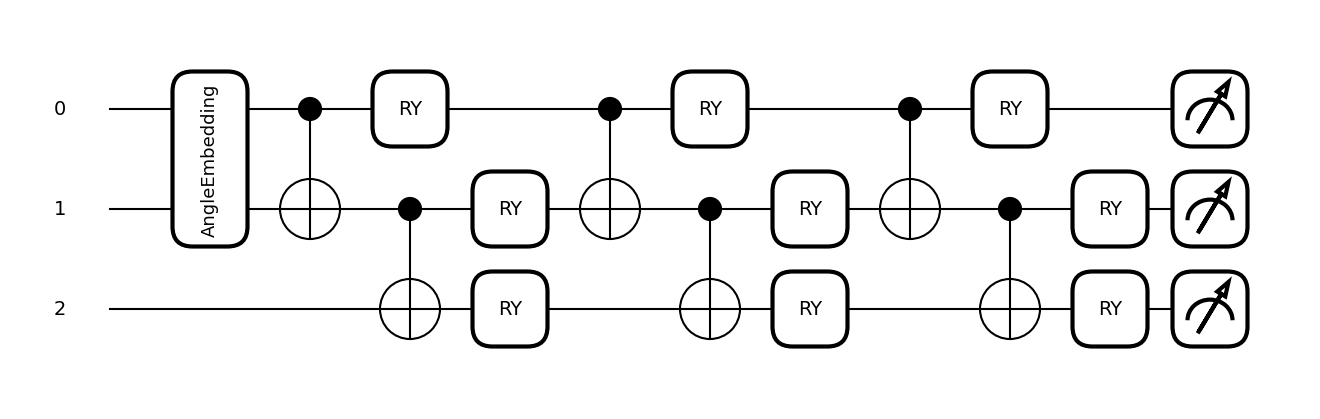
\includegraphics[width=0.8\textwidth]{figs/pqc_2d}\
                \caption{2-d image quantum circuit 구조}
                \label{fig:2d-image}
                \end{figure}

                이러한 모델은, 우리는 사진 3장(256x256)에 대하여, reconstruction error를 PSNR metric를 사용하여 학습된 성능을 평가하였다. PSNR의 수식은 다음과 같이 정의 된다.이는 높은 PSNR이 더 잘 reconstruction함을 뜻한다.

                \[
                    \text{PSNR} = 10 \cdot \log_{10}\left(\frac{\text{MAX}_I^2}{\text{MSE}}\right)
                    \]

                이와 같은 방법으로, 여러 layer별로 성능차이를 비교해보았으며, 결과는 다음과 같이 나타났다.

                \begin{table}[ht]
                    \centering
                    \begin{tabular}{c|ccc}
                    \Xhline{3\arrayrulewidth}
                    \multirow{2}{*}{Layers} & \multicolumn{3}{c}{PSNR (dB)} \\
                    \cline{2-4}
                    & Image 1 & Image 2 & Image 3 \\
                    \hline
                    MLP (1 layer) & 24.3 & 23.8 & 24.1 \\
                    MLP (2 layers) & 25.7 & 25.2 & 25.5 \\
                    MLP (3 layers) & 26.4 & 26.1 & 26.3 \\
                    \hline
                    PQC (1 layer) & 25.1 & 24.9 & 25.0 \\
                    PQC (2 layers) & 26.8 & 26.5 & 26.7 \\
                    PQC (3 layers) & 27.9 & 27.6 & 27.8 \\
                    \Xhline{3\arrayrulewidth}
                    \end{tabular}
                    \caption{PSNR comparison between MLP and QML models across different layer configurations}
                    \label{tab:psnr_comparison}
                \end{table}

        \item \textbf{1-d function estimation} :
본 태스크는 1차원 입력 x를 받아 스칼라 값 y를 예측하는 문제이다. 모델은 입력 x에 대해 출력 y를 예측하며, 예측된 값과 실제 값 간의 손실을 계산하여 학습을 진행한다. 이를 수식으로 표현하면 다음과 같다:

\[
\text{Input}: x \in \mathbb{R}
\]

\[
\text{Prediction}: \hat{y} = f(x; \theta)
\]

\[
\text{Loss Function}: \mathcal{L}(\theta) = \frac{1}{N} \sum_{i=1}^{N} (\hat{y}_i - y_i)^2
\]

여기서 \(f\)는 모델 함수, \(\theta\)는 모델의 파라미터, \(N\)은 데이터 샘플의 수를 나타낸다. 모델은 손실 함수를 최소화하도록 파라미터 \(\theta\)를 최적화하여 예측된 값이 실제 값과 잘 일치하도록 학습된다. ML과 QML의 차이는 모델과 데이터 인코딩에서만 차이나는데, 각각 다음과 같이 진행된다.


\begin{table}[ht]
    \centering
    \begin{tabular}{ l||p{5.5cm}||p{5.5cm}}
    \Xhline{3\arrayrulewidth}
    \textbf{Item} & \textbf{MLP} & \textbf{QML} \\
    \hline
    Data Encoding & $x \in \mathbb{R}$을 $[-1, 1]$ 사이로 정규화하였다. &
    Angle Encoding을 사용하였다. $x \in \mathbb{R}$을 $[-1, 1]$ 사이로 정규화한 이후, 이 값을 2개의 qubit 중 첫 번째 qubit의 RX gate에 $\theta_x$를 $[-\pi, \pi]$ 값 사이에 위치하도록 정규화하여 Angle encoding 하였다. \\
    \hline
    Model & MLP 모델을 사용하였으며, 입력 레이어 1개, 히든 레이어 2개, 출력 레이어 1개로 구성하였으며, activation function은 RELU를 사용하였다. &
    2개의 qubit을 사용하였고, $\prod_{0}^{1} RY_i(\theta)CX_i$의 gate를 3번 반복함으로써 3층의 레이어의 효과가 나타나도록 구현하였다.이를 다음과 같이 시각화하였다.\labelcref{fig:1d-image} \\
    \Xhline{3\arrayrulewidth}
    \end{tabular}
    \caption{MLP와 QML의 비교}
    \label{tab:mlp_qml_comparison_1d}
\end{table}

\begin{figure}[h]
    \centering
    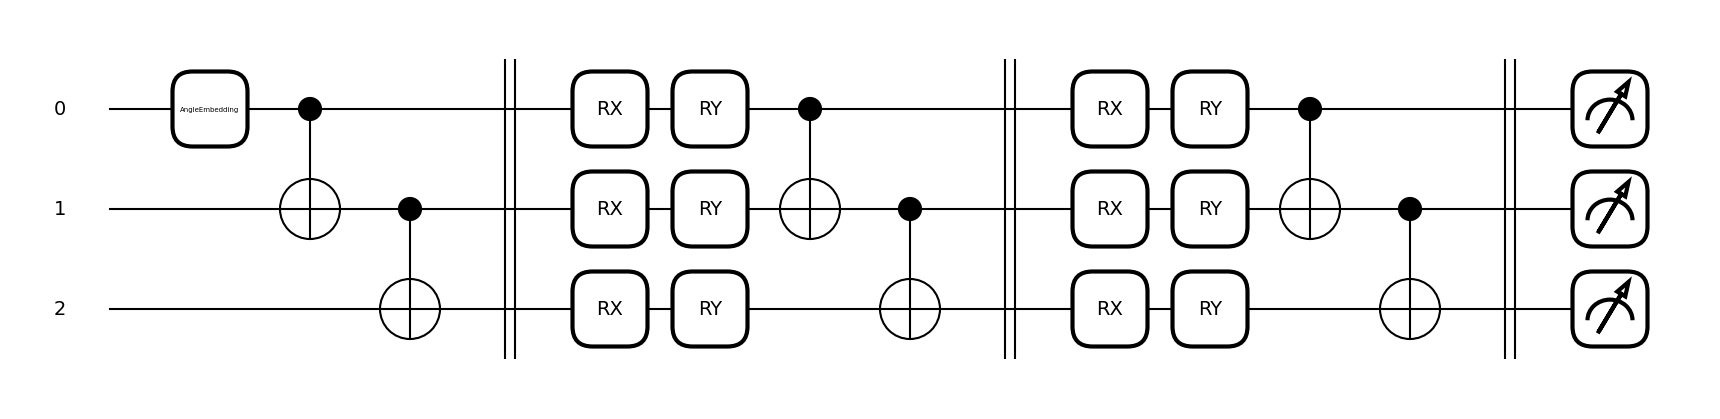
\includegraphics[width=0.8\textwidth]{figs/pqc_1d}\
\caption{1-d image quantum circuit 구조}
\label{fig:1d-image}
\end{figure}
\end{itemize}

이 실험또한 마찬가지로, 여러 레이어의 개수로 실험하였고, 다양성을 위해 3 개의 함수에서 MSE  결과를 측정하였다.
\begin{table}[ht]
    \centering
    \begin{tabular}{c|ccc}
    \Xhline{3\arrayrulewidth}
    \multirow{2}{*}{Layers} & \multicolumn{3}{c}{MSE} \\
    \cline{2-4}
    & $sin(x)$  & $tanh(x)$ & $x$ \\
    \hline
    MLP (1 layer) & 24.3 & 23.8 & 24.1 \\
    MLP (2 layers) & 25.7 & 25.2 & 25.5 \\
    MLP (3 layers) & 26.4 & 26.1 & 26.3 \\
    \hline
    PQC (1 layer) & 25.1 & 24.9 & 25.0 \\
    PQC (2 layers) & 26.8 & 26.5 & 26.7 \\
    PQC (3 layers) & 27.9 & 27.6 & 27.8 \\
    \Xhline{3\arrayrulewidth}
    \end{tabular}
    \caption{MSEcomparison between MLP and QML models across different layer configurations}
    \label{tab:mse_comparison}
\end{table}




\section{Limitations of QML: Constraint of Nonlinearity}

3.3 장에서 살펴본 결과, QML이 2d, 1d에서 잘 작동하지 않는 것을 확인하였다. 이에 대한 이유를 quantum circuit의 비선형성의 부족으로 유추하였다. 이를 수학적으로 분석하기 위해, QML의 circuit 구조에 따라, input에서 output까지 나오게 되는 과정을 수식화하였다.2-qubit 상태일때의 input과 output의 관계를 수식화 하면 다음과 같다.
먼저, 2-qubit 시스템에서의 초기 상태를 다음과 같이 나타낼 수 있다:

\[
|\psi_0\rangle = |0\rangle \otimes |0\rangle = \begin{pmatrix} 1 \\ 0 \\ 0 \\ 0 \end{pmatrix}
\]

이에 \labelcref{fig:2d-image} circuit을 통관 후의 상태를 다음과 같이 나타낼수 있다.

\[
|\psi_1\rangle = CX \cdot (RY(\theta_2) \otimes RY(\theta_1)) \cdot (RX(x) \otimes I_2) \cdot |\psi_0\rangle
\]

최종 출력값은 측정 연산자 Z를 통해 얻어지며:

\[
\text{output} = \langle\psi_1|Z|\psi_1\rangle = \langle\psi_1|\begin{pmatrix} 1 & 0 \\ 0 & -1 \end{pmatrix}|\psi_1\rangle
\]

이 전체 과정은 입력 x에 대해 선형 변환들의 연속적인 적용으로 이루어지며, 측정 과정에서만 제한된 비선형성이 도입됨을 알 수 있다. 이에 우리는 QRF에 적용된 비선형 Q-RELU를 적용하였으나,이마저 성능이 향상되지 않았다. 이 이유에 대해서는 reference를 참조하여,
알게되었고, 이에 새로운 형태의 비선형 circuit 이 필요함을 느끼게되었다.






% You may modify the preference settings at the preamble in the ``\texttt{manuscript.tex}'' file.